% Created 2023-01-29 dom 12:20
% Intended LaTeX compiler: pdflatex
\documentclass[aspectratio=169, usenames,svgnames,dvipsnames]{beamer}
\usepackage[utf8]{inputenc}
\usepackage[T1]{fontenc}
\usepackage{graphicx}
\usepackage{longtable}
\usepackage{wrapfig}
\usepackage{rotating}
\usepackage[normalem]{ulem}
\usepackage{amsmath}
\usepackage{amssymb}
\usepackage{capt-of}
\usepackage{hyperref}
\usepackage{color}
\usepackage{listings}
\usepackage{mathpazo}
\usepackage{gensymb}
\usepackage{amsmath}
\usepackage{diffcoeff}
\usepackage{steinmetz}
\usepackage{mathtools}
\bibliographystyle{plain}
\usepackage{siunitx}
\sisetup{output-decimal-marker={,}}
\DeclareSIUnit{\watthour}{Wh}
\hypersetup{colorlinks=true, linkcolor=Blue, urlcolor=Blue}
\renewcommand{\thefootnote}{\fnsymbol{footnote}}
\newcommand{\laplace}[1]{\mathbf{#1}(\mathbf{s})}
\newcommand{\slp}{\mathbf{s}}
\newcommand{\fasor}[1]{\mathbf{#1}(\omega)}
\newcommand{\atan}{\mathrm{atan}}
\parskip=5pt
\usetheme{Boadilla}
\usecolortheme{rose}
\usefonttheme{serif}
\author{Oscar Perpiñán Lamigueiro}
\date{}
\title{Sistemas Trifásicos}
\subtitle{Teoría de Circuitos II}
\setbeamercolor{alerted text}{fg=blue!50!black} \setbeamerfont{alerted text}{series=\bfseries}
\AtBeginSubsection[]{\begin{frame}[plain]\tableofcontents[currentsubsection,sectionstyle=show/shaded,subsectionstyle=show/shaded/hide]\end{frame}}
\AtBeginSection[]{\begin{frame}[plain]\tableofcontents[currentsection,hideallsubsections]\end{frame}}
\beamertemplatenavigationsymbolsempty
\setbeamertemplate{footline}[frame number]
\setbeamertemplate{itemize items}[triangle]
\setbeamertemplate{enumerate items}[circle]
\setbeamertemplate{section in toc}[circle]
\setbeamertemplate{subsection in toc}[circle]
\hypersetup{
 pdfauthor={Oscar Perpiñán Lamigueiro},
 pdftitle={Sistemas Trifásicos},
 pdfkeywords={},
 pdfsubject={},
 pdfcreator={Emacs 28.2 (Org mode 9.6)}, 
 pdflang={Spanish}}
\begin{document}

\maketitle

\section{Generadores}
\label{sec:org2fef522}
\begin{frame}[label={sec:orgcfb0058}]{Tensiones de Fase y Línea}
\begin{columns}
\begin{column}{0.4\columnwidth}
\begin{center}
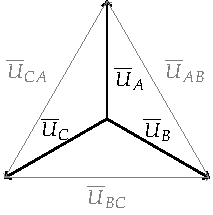
\includegraphics[height=0.4\textheight]{../figs/FasoresTrifasica_ABC.pdf}
\end{center}
\end{column}

\begin{column}{0.6\columnwidth}
Tensiones de \alert{Fase}: \(U_A\), \(U_B\), \(U_C\)

Tensiones de \alert{Línea}: \(U_{AB}\), \(U_{BC}\), \(U_{CA}\)
\end{column}
\end{columns}

     \begin{align*}
       \overline{U}_{AB} &= \overline{U}_A - \overline{U}_B\\
       \overline{U}_{BC} &= \overline{U}_B - \overline{U}_C\\
       \overline{U}_{CA} &= \overline{U}_C - \overline{U}_A\\
\cline{1-2}
       \overline{U}_{AB} + \overline{U}_{BC} + \overline{U}_{CA} &= 0     \end{align*}
\end{frame}

\begin{frame}[label={sec:org811489d}]{Tensiones de Fase y Línea}
\begin{columns}
\begin{column}{0.5\columnwidth}
\begin{align*}
  \overline{U}_A &= U_f\phase{\theta_f}\\
  \overline{U}_B &= U_f\phase{\theta_f - \ang{120}}
\end{align*}

\begin{align*}
\overline{U}_{AB} &= \overline{U}_A - \overline{U}_B = \\
		  &= U_f\phase{\theta_f} - U_f\phase{\theta_f - \ang{120}} = \\
		  &= U_f\phase{\theta_f} + U_f\phase{\theta_f + \ang{60}}\\
		  &= 2 \cdot U_f \cdot \cos(30) \phase{\theta_f + \ang{30}} = \\
  &= \sqrt{3} U_f \phase{\theta_f + \ang{30}}
\end{align*}
\end{column}

\begin{column}{0.5\columnwidth}
\begin{center}
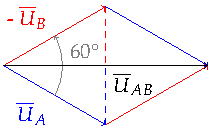
\includegraphics[width=.9\linewidth]{../figs/FasoresFaseLinea.pdf}
\end{center}

\[
  \boxed{
    \begin{array}{l}
      U = \sqrt{3}\cdot U_f\\
      \theta_l = \theta_f + \ang{30}\\
    \end{array}
  }
\]
\end{column}
\end{columns}
\end{frame}
\begin{frame}[label={sec:org38bed21}]{Secuencia de Fases}
\begin{itemize}
\item Sentido en el que ocurren los máximos de cada fase.
\item Secuencia de Fases Directa (\alert{SFD}): ABC
\end{itemize}
\begin{center}
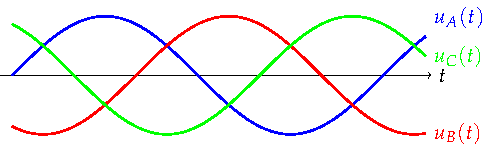
\includegraphics[height=0.3\textheight]{../figs/TensionesTrifasica_ABC.pdf}
\end{center}
\begin{itemize}
\item Secuencia de Fases Inversa (\alert{SFI}): ACB
\end{itemize}
\begin{center}
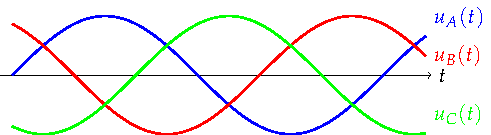
\includegraphics[height=0.3\textheight]{../figs/TensionesTrifasica_ACB.pdf}
\end{center}
\end{frame}

\begin{frame}[label={sec:org1c63bce}]{Secuencia de Fases Directa (SFD)}
\begin{center}
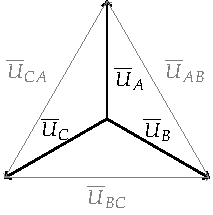
\includegraphics[height=0.45\textheight]{../figs/FasoresTrifasica_ABC.pdf}
\end{center}

\begin{columns}
\begin{column}{0.4\columnwidth}
\begin{align*}
  \overline{U}_A &= \frac{U}{\sqrt{3}}\phase{{\color{blue}\ang{90}}}\\
  \overline{U}_B &= \frac{U}{\sqrt{3}}\phase{\ang{-30}}\\
  \overline{U}_C &= \frac{U}{\sqrt{3}}\phase{\ang{-150}}
\end{align*}
\end{column}
\begin{column}{0.2\columnwidth}
\begin{center}
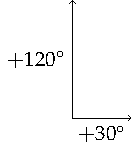
\includegraphics[width=.9\linewidth]{../figs/ReglaSFD.pdf}
\end{center}
\end{column}

\begin{column}{0.4\columnwidth}
\begin{align*}
  \overline{U}_{AB} &= U\phase{\ang{120}}\\
  \overline{U}_{BC} &= U\phase{{\color{blue}\ang{0}}}\\
  \overline{U}_{CA} &= U\phase{\ang{-120}}
\end{align*}
\end{column}
\end{columns}
\end{frame}


\begin{frame}[label={sec:org2acbb89}]{Secuencia de Fases Inversa (SFI)}
\begin{center}
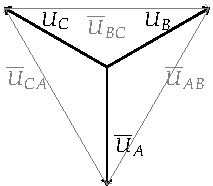
\includegraphics[height=0.45\textheight]{../figs/FasoresTrifasica_ACB.pdf}
\end{center}
\begin{columns}
\begin{column}{0.4\columnwidth}
\begin{align*}
  \overline{U}_A &= \frac{U}{\sqrt{3}}\phase{{\color{blue}\ang{-90}}}\\
  \overline{U}_B &= \frac{U}{\sqrt{3}}\phase{\ang{30}}\\
  \overline{U}_C &= \frac{U}{\sqrt{3}}\phase{\ang{150}}
\end{align*}
\end{column}

\begin{column}{0.2\columnwidth}
\begin{center}
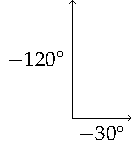
\includegraphics[width=.9\linewidth]{../figs/ReglaSFI.pdf}
\end{center}
\end{column}
\begin{column}{0.4\columnwidth}
\begin{align*}
  \overline{U}_{AB} &= U\phase{\ang{-120}}\\
  \overline{U}_{BC} &= U\phase{{\color{blue}\ang{0}}}\\
  \overline{U}_{CA} &= U\phase{\ang{120}}
\end{align*}
\end{column}
\end{columns}
\end{frame}
\section{Receptores}
\label{sec:orgcc3d1f7}
\begin{frame}[label={sec:org498c373}]{Tipos de Receptores}
\begin{block}{Conexión}
\begin{itemize}
\item \alert{Estrella} (punto común) Y
\item \alert{Triángulo} \(\triangle\)
\end{itemize}
\end{block}

\begin{block}{Impedancias}
\begin{itemize}
\item \alert{Equilibrado} (las tres impedancias son idénticas en módulo \alert{y} fase).
\item \alert{Desequilibrado}
\end{itemize}
\end{block}
\end{frame}


\begin{frame}[label={sec:org8ca0b2e}]{Receptor en Estrella Equilibrado}
\begin{columns}
\begin{column}{0.5\columnwidth}
\begin{center}
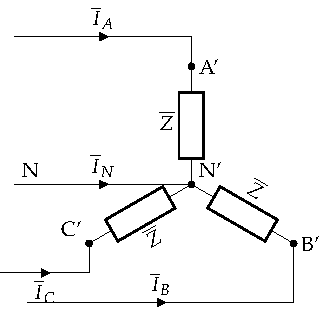
\includegraphics[width=.9\linewidth]{../figs/EstrellaEquilibrado_Receptor.pdf}
\end{center}
\end{column}

\begin{column}{0.5\columnwidth}
\begin{align*}
  \overline{I}_A &= \frac{\overline{U}_A}{\overline{Z}} = \frac{U_f}{Z}\phase{\ang{\pm 90} - \theta} \\
  \overline{I}_B &= \frac{\overline{U}_B}{\overline{Z}} = \frac{U_f}{Z}\phase{\ang{\mp 30} - \theta}\\
  \overline{I}_C &= \frac{\overline{U}_C}{\overline{Z}} = \frac{U_f}{Z}\phase{\ang{\mp 150} - \theta}
\end{align*}


\[
  \boxed{|\overline{I}_A| = |\overline{I}_B| = |\overline{I}_C| = \frac{U_f}{Z}}
\]

\[
  \overline{I}_A  + \overline{I}_B + \overline{I}_C + \overline{I}_N = 0
\]
\[
   \overline{I}_A  + \overline{I}_B + \overline{I}_C  = 0 \rightarrow \boxed{\overline{I}_N = 0}
\]
\end{column}
\end{columns}
\end{frame}
\begin{frame}[label={sec:orgfa7b248}]{Receptor en Estrella Equilibrado}
\begin{center}
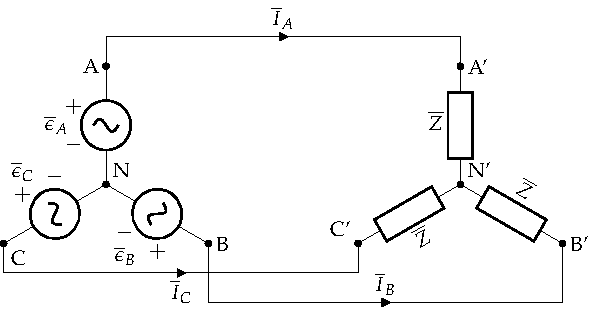
\includegraphics[width=.9\linewidth]{../figs/EstrellaEquilibrado_SinNeutro.pdf}
\end{center}
\end{frame}

\begin{frame}[label={sec:org0451afc}]{Receptor en Triángulo Equilibrado}
\begin{columns}
\begin{column}{0.5\columnwidth}
\begin{center}
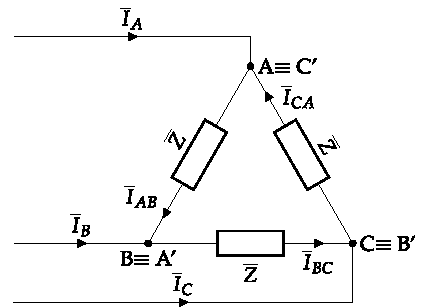
\includegraphics[width=.9\linewidth]{../figs/TrianguloEquilibrado_Receptor.pdf}
\end{center}
\end{column}

\begin{column}{0.5\columnwidth}
\begin{align*}
  \overline{I}_{AB} &= \frac{\overline{U}_{AB}}{\overline{Z}} = \frac{U}{Z}\phase{\ang{\pm 120} - \theta} \\
  \overline{I}_{BC} &= \frac{\overline{U}_{BC}}{\overline{Z}} = \frac{U}{Z}\phase{0 - \theta}\\
  \overline{I}_{CA} &= \frac{\overline{U}_{CA}}{\overline{Z}} = \frac{U}{Z}\phase{\ang{\mp 120} - \theta}
\end{align*}

\[
   \overline{I}_{AB}  + \overline{I}_{BC} + \overline{I}_{CA}  = 0 
\]

Corriente de Fase:
\[
  \boxed{I_f = |\overline{I}_{AB}| = |\overline{I}_{BC}| = |\overline{I}_{CA}| = \frac{U}{Z}}
\]
\end{column}
\end{columns}
\end{frame}


\begin{frame}[label={sec:orgcf870ac}]{Receptor en Triángulo Equilibrado}
\begin{columns}
\begin{column}{0.5\columnwidth}
\begin{center}
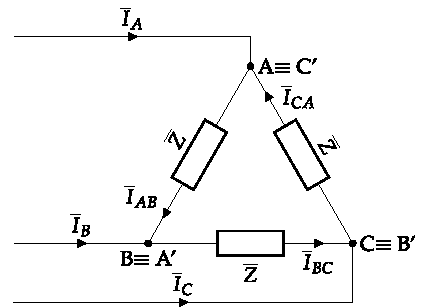
\includegraphics[width=.9\linewidth]{../figs/TrianguloEquilibrado_Receptor.pdf}
\end{center}
\end{column}

\begin{column}{0.5\columnwidth}
\begin{align*}
  \overline{I}_A &= \overline{I}_{AB} - \overline{I}_{CA} = \sqrt{3} \cdot \frac{U}{Z}\phase{\ang{\pm 90} - \theta}\\
  \overline{I}_B &= \overline{I}_{BC} - \overline{I}_{AB} = \sqrt{3} \cdot \frac{U}{Z}\phase{\ang{\mp 30} - \theta}\\
  \overline{I}_C &= \overline{I}_{CA} - \overline{I}_{BC} = \sqrt{3} \cdot \frac{U}{Z}\phase{\ang{\mp 150} - \theta}\\
\end{align*}

Corriente de Línea:
\[
  \boxed{I = |\overline{I}_A| = |\overline{I}_B| = |\overline{I}_C| = \sqrt{3} \cdot \frac{U}{Z}}
\]

\[
  \boxed{I = \sqrt{3} \cdot I_f}
\]
\end{column}
\end{columns}
\end{frame}

\begin{frame}[label={sec:org47f0049}]{Receptor en Estrella Desequilibrado con Neutro}
\begin{columns}
\begin{column}{0.5\columnwidth}
\begin{center}
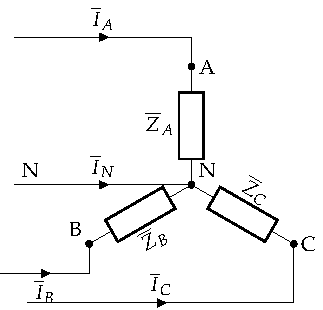
\includegraphics[width=.9\linewidth]{../figs/EstrellaDesequilibrado_Receptor.pdf}
\end{center}
\end{column}

\begin{column}{0.5\columnwidth}
\begin{align*}
  \overline{I}_A &= \frac{\overline{U}_A}{\overline{Z}_A}\\
  \overline{I}_B &= \frac{\overline{U}_B}{\overline{Z}_B}\\
  \overline{I}_C &= \frac{\overline{U}_C}{\overline{Z}_C}
\end{align*}

\[
  \overline{I}_A  + \overline{I}_B + \overline{I}_C + \overline{I}_N = 0
\]
\[
   \overline{I}_A  + \overline{I}_B + \overline{I}_C  \neq 0 \rightarrow \boxed{\overline{I}_N \neq 0}
\]
\end{column}
\end{columns}
\end{frame}

\begin{frame}[label={sec:org77bc54f}]{Receptor en Estrella Desequilibrado sin Neutro}
\begin{center}
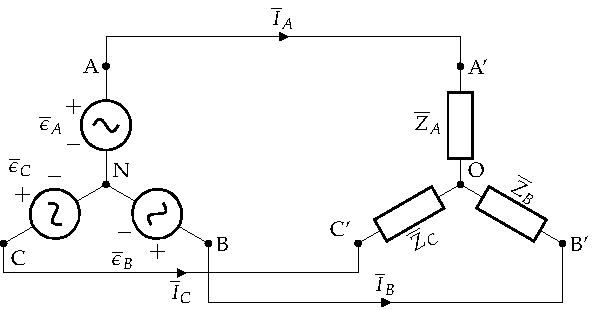
\includegraphics[width=.9\linewidth]{../figs/EstrellaDesequilibrado_SinNeutro.pdf}
\end{center}

\[
\overline{U}_N \neq \overline{U}_{N'}
\]
\end{frame}

\begin{frame}[label={sec:org2e515bc}]{Método del desplazamiento del neutro}
Ecuaciones del receptor:
\begin{align*}
  \overline{U}_{A'N'} &= \overline{I}_A \cdot \overline{Z}_A\\
  \overline{U}_{B'N'} &= \overline{I}_B \cdot \overline{Z}_B\\
  \overline{U}_{C'N'} &= \overline{I}_C \cdot \overline{Z}_C
\end{align*}
Ecuación del nudo \(N'\):
\[
  \overline{I}_A + \overline{I}_B + \overline{I}_C = 0
\]
\end{frame}

\begin{frame}[label={sec:orgd35af0a}]{Método del desplazamiento del neutro}
Relacionamos las tensiones en el receptor con las tensiones del generador:
\begin{align*}
  \overline{U}_{A'N'} &= \overline{U}_{AN} - \overline{U}_{NN'}\\
  \overline{U}_{B'N'} &= \overline{U}_{BN} - \overline{U}_{NN'}\\
  \overline{U}_{C'N'} &= \overline{U}_{CN} - \overline{U}_{NN'}
\end{align*}

Despejamos las corrientes teniendo en cuenta estas relaciones:
\begin{align*}
  \overline{I}_A &= \frac{\overline{U}_{AN} - \overline{U}_{NN'}}{\overline{Z}_A}\\
  \overline{I}_B &= \frac{\overline{U}_{AN} - \overline{U}_{NN'}}{\overline{Z}_B}\\
  \overline{I}_C &= \frac{\overline{U}_{AN} - \overline{U}_{NN'}}{\overline{Z}_C}
\end{align*}
\end{frame}

\begin{frame}[label={sec:orgedd4627}]{Método del desplazamiento del neutro}
Finalmente, usando la ecuación del nudo \(N'\) despejamos la tensión \(U_{N'N}\) (tensión de desplazamiento del neutro)\footnote{Se puede llegar a este mismo resultado aplicando el teorema de Millman.}:

\[
  \boxed{\overline{U}_{N'N} = \frac{\overline{U}_{AN} \cdot \overline{Y}_A + \overline{U}_{BN} \cdot \overline{Y}_B + \overline{U}_{CN} \cdot \overline{Y}_C}{\overline{Y}_A + \overline{Y}_B + \overline{Y}_C}}
\]

Una vez calculada esta tensión \(\overline{U}_{N'N}\) se pueden calcular las corrientes de línea.
\end{frame}
\begin{frame}[label={sec:org09f1d2d}]{Receptor en Estrella con Carga Monofásica}
\begin{center}
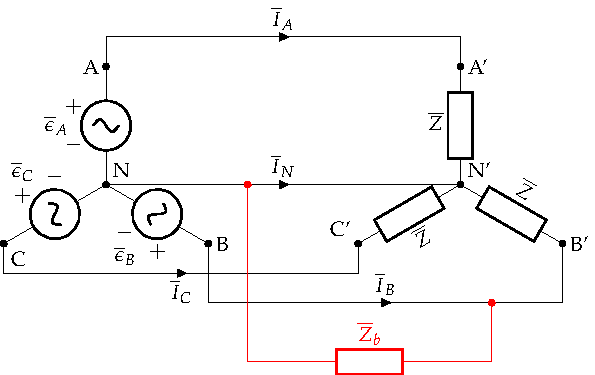
\includegraphics[height=0.9\textheight]{../figs/Estrella_CargaMonofasica.pdf}
\end{center}
\end{frame}
\begin{frame}[label={sec:orgc1ab7c3}]{Receptor en Triángulo Desequilibrado}
\begin{columns}
\begin{column}{0.6\columnwidth}
\begin{center}
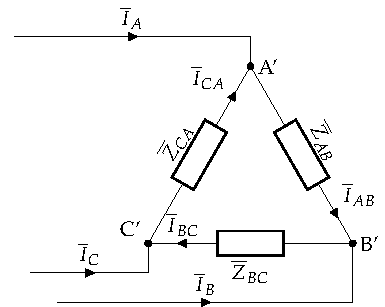
\includegraphics[width=.9\linewidth]{../figs/TrianguloDesequilibrado_Receptor.pdf}
\end{center}
\end{column}

\begin{column}{0.4\columnwidth}
\begin{align*}
  \overline{I}_{AB} &= \frac{\overline{U}_{AB}}{\overline{Z}_{AB}}\\
  \overline{I}_{BC} &= \frac{\overline{U}_{BC}}{\overline{Z}_{BC}}\\
  \overline{I}_{CA} &= \frac{\overline{U}_{CA}}{\overline{Z}_{CA}}
\end{align*}

\begin{align*}
  \overline{I}_A &= \overline{I}_{AB} - \overline{I}_{CA}\\
  \overline{I}_B &= \overline{I}_{BC} - \overline{I}_{AB}\\
  \overline{I}_C &= \overline{I}_{CA} - \overline{I}_{BC}\\
\end{align*}
\end{column}
\end{columns}
\end{frame}

\section{Potencia en Sistemas Trifásicos}
\label{sec:org17f0636}

\begin{frame}[label={sec:orgd5cad97}]{Receptor en Estrella Equilibrado}
\begin{columns}
\begin{column}{0.5\columnwidth}
\begin{center}
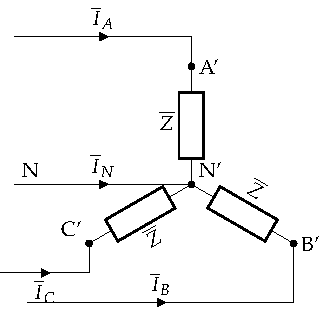
\includegraphics[width=.9\linewidth]{../figs/EstrellaEquilibrado_Receptor.pdf}
\end{center}
\end{column}

\begin{column}{0.5\columnwidth}
\begin{align*}
  P = 3 \cdot P_Z &= 3 \cdot U_Z I_Z \cos(\theta)\\
  Q = 3 \cdot Q_Z &= 3 \cdot U_Z I_Z \sin(\theta)
\end{align*}

\begin{align*}
  I_Z &= I\\
  U_Z &= U_F
\end{align*}


\begin{align*}
  P &= 3 U_F I \cos(\theta) = \sqrt{3} U I \cos(\theta)\\
  Q &= 3 U_F I \sin(\theta) = \sqrt{3} U I \sin(\theta)\\
  S &= \sqrt{P^2 + Q^2} =  \sqrt{3} U I
\end{align*}
\end{column}
\end{columns}
\end{frame}


\begin{frame}[label={sec:org9751122}]{Receptor en Triángulo Equilibrado}
\begin{columns}
\begin{column}{0.5\columnwidth}
\begin{center}
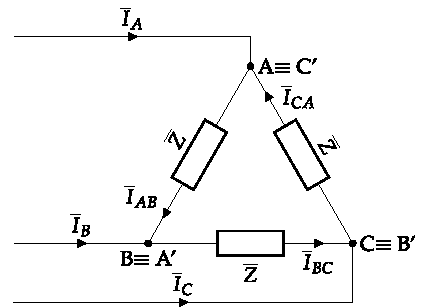
\includegraphics[width=.9\linewidth]{../figs/TrianguloEquilibrado_Receptor.pdf}
\end{center}
\end{column}

\begin{column}{0.5\columnwidth}
\begin{align*}
  P = 3 \cdot P_Z &= 3 \cdot U_Z I_Z \cos(\theta)\\
  Q = 3 \cdot Q_Z &= 3 \cdot U_Z I_Z \sin(\theta)
\end{align*}

\begin{align*}
  I_Z &= I_F\\
  U_Z &= U
\end{align*}


\begin{align*}
  P &= 3 U I_F \cos(\theta) = \sqrt{3} U I \cos(\theta)\\
  Q &= 3 U I_F \sin(\theta) = \sqrt{3} U I \sin(\theta)\\
  S &= \sqrt{P^2 + Q^2} =  \sqrt{3} U I
\end{align*}
\end{column}
\end{columns}
\end{frame}

\begin{frame}[label={sec:orgf80ede4}]{Receptor en Estrella Desequilibrado}
\begin{columns}
\begin{column}{0.5\columnwidth}
\begin{center}
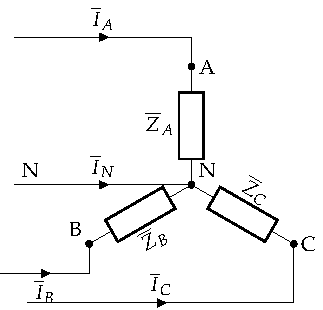
\includegraphics[width=.9\linewidth]{../figs/EstrellaDesequilibrado_Receptor.pdf}
\end{center}
\end{column}

\begin{column}{0.5\columnwidth}
\begin{align*}
  P &= P_A + P_B + P_C\\
  Q &= Q_A + Q_B + Q_C\\
  \overline{S} &= P + jQ
\end{align*}
\end{column}
\end{columns}
\end{frame}

\begin{frame}[label={sec:org960add6}]{Receptor en Triángulo Desequilibrado}
\begin{columns}
\begin{column}{0.6\columnwidth}
\begin{center}
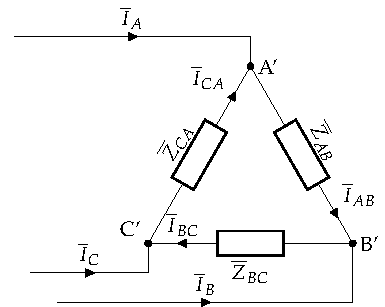
\includegraphics[width=.9\linewidth]{../figs/TrianguloDesequilibrado_Receptor.pdf}
\end{center}
\end{column}

\begin{column}{0.4\columnwidth}
\begin{align*}
  P &= P_{AB} + P_{BC} + P_{CA}\\
  Q &= Q_{AB} + Q_{BC} + Q_{CA}\\
  \overline{S} &= P + jQ
\end{align*}
\end{column}
\end{columns}
\end{frame}

\section{Compensación de Reactiva}
\label{sec:orgd65e800}

\begin{frame}[label={sec:org143c6c7}]{Conexión en Triángulo}
\begin{columns}
\begin{column}{0.5\columnwidth}
\begin{center}
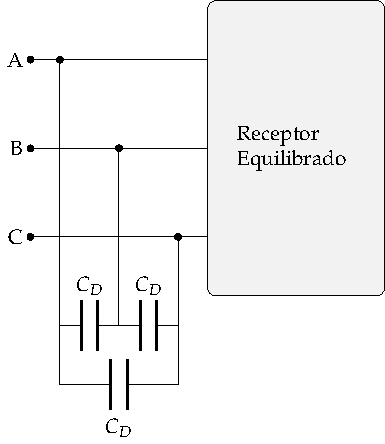
\includegraphics[width=.9\linewidth]{../figs/CircuitoTrifasica_CompensacionReactiva.pdf}
\end{center}
\end{column}

\begin{column}{0.5\columnwidth}
\begin{align*}
  Q &= P\tan\theta\\
  Q' &= P\tan\theta' =\\
    &= Q - Q_c\\
  Q_c &= 3 \cdot \omega C_\triangle \cdot U^2
\end{align*}
\[
  \boxed{C_\triangle = \frac{P(\tan \theta - \tan \theta')}{3\omega U^2}}
\]
\end{column}
\end{columns}
\end{frame}

\begin{frame}[label={sec:orgb2929b1}]{Conexión en Estrella}
\begin{columns}
\begin{column}{0.5\columnwidth}
\begin{center}
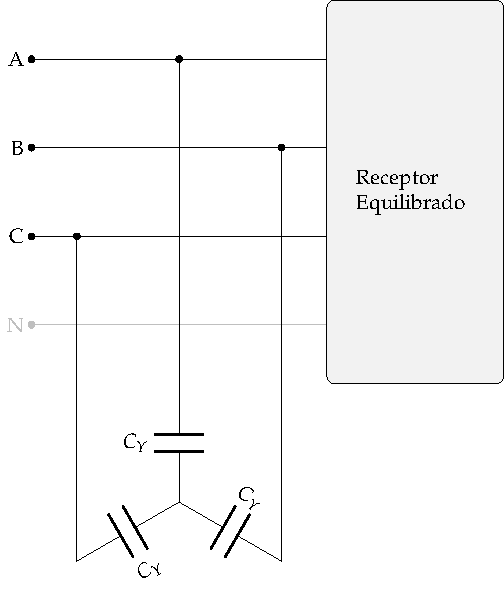
\includegraphics[width=.9\linewidth]{../figs/CircuitoTrifasicaY_CompensacionReactiva.pdf}
\end{center}
\end{column}
\begin{column}{0.5\columnwidth}
\begin{align*}
  Q &= P\tan\theta\\
  Q' &= P\tan\theta' =\\
    &= Q - Q_c\\
  Q_c &= 3 \cdot \omega C_Y \cdot U_f^2
\end{align*}
\[
  \boxed{C_Y = \frac{P(\tan \theta - \tan \theta')}{\omega U^2}}
\]
\end{column}
\end{columns}
\end{frame}
\begin{frame}[label={sec:orgec4fa80}]{Comparación Estrella-Triángulo}
\begin{columns}
\begin{column}{0.5\columnwidth}
\begin{center}
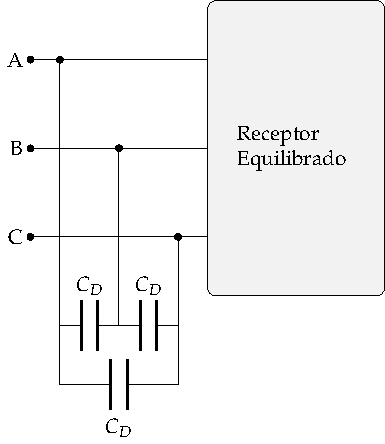
\includegraphics[height=0.55\textheight]{../figs/CircuitoTrifasica_CompensacionReactiva.pdf}
\end{center}
\[
  \boxed{C_\triangle = \frac{P(\tan \theta - \tan \theta')}{3 \omega U^2}}
\]
\end{column}

\begin{column}{0.5\columnwidth}
\begin{center}
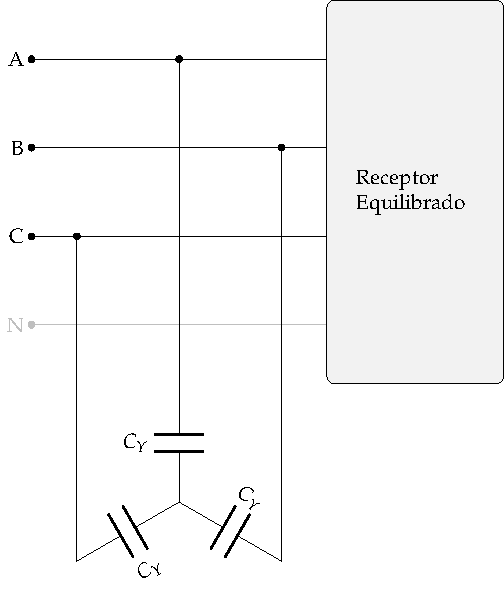
\includegraphics[height=0.55\textheight]{../figs/CircuitoTrifasicaY_CompensacionReactiva.pdf}
\end{center}
\[
  \boxed{C_Y = \frac{P(\tan \theta - \tan \theta')}{\omega U^2}}
\]

\medskip
\end{column}
\end{columns}

Dado que \(C_Y = 3 \cdot C_\triangle\) la \alert{configuración recomendada} es \alert{triángulo}.
\end{frame}
\section{Medida de Potencia en Sistemas Trifásicos}
\label{sec:org4a24397}
\begin{frame}[label={sec:orge4a291e}]{Recordatorio: vatímetro}
\begin{center}
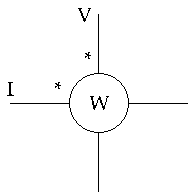
\includegraphics[height=0.6\textheight]{../figs/vatimetro.pdf}
\end{center}

\alert{Vatímetro}: equipo de medida de 4 terminales (1 par para tensión, 1 par para corriente)

\[
  \boxed{W = \Re(\overline{U} \cdot \overline{I}^*)}
\]
\end{frame}
\begin{frame}[label={sec:org638b00a}]{Sistema de 4 Hilos}
\begin{columns}
\begin{column}{0.7\columnwidth}
\begin{center}
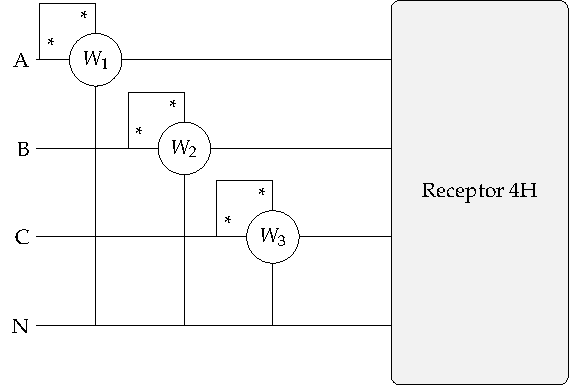
\includegraphics[height=0.85\textheight]{../figs/Potencia4H.pdf}
\end{center}
\end{column}

\begin{column}{0.3\columnwidth}
\begin{align*}
  W_1 &= \Re(\overline{U}_A \cdot \overline{I}_A^*) = P_A\\
  W_2 &= \Re(\overline{U}_B \cdot \overline{I}_B^*) = P_B\\
  W_3 &= \Re(\overline{U}_C \cdot \overline{I}_C^*) = P_C\\
\end{align*}

\[
  \boxed{P = W_1 + W_2 + W_3}
\]
\end{column}
\end{columns}
\end{frame}


\begin{frame}[label={sec:orge7fb9d3}]{Sistema de 3 Hilos Equilibrado}
\begin{center}
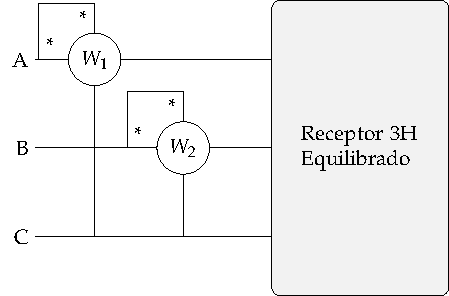
\includegraphics[height=0.3\textheight]{../figs/Potencia3H_Equilibrado_AB.pdf}
\end{center}

\begin{columns}
\begin{column}{0.5\columnwidth}
SFD
\begin{align*}
  W_1 &= UI\cos(\theta {\color{red}-} \ang{30})\\
  W_2 &= UI\cos(\theta {\color{red}+} \ang{30})
\end{align*}
\begin{align*}
  P &= W_1 + W_2\\
  Q &= \sqrt{3}({\color{red}W_1 - W_2}) \\
  \tan\theta &= \sqrt{3} \frac{{\color{red}W_1 - W_2}}{W_1 + W_2}
\end{align*}
\end{column}
\begin{column}{0.5\columnwidth}
SFI
\begin{align*}
  W_1 &= UI\cos(\theta {\color{red}+} \ang{30})\\
  W_2 &= UI\cos(\theta {\color{red}-} \ang{30})
\end{align*}
\begin{align*}
  P &= W_1 + W_2\\
  Q &= \sqrt{3}({\color{red}W_2 - W_1}) \\
  \tan\theta &= \sqrt{3} \frac{{\color{red}W_2 - W_1}}{W_1 + W_2}
\end{align*}
\end{column}
\end{columns}
\end{frame}
\begin{frame}[label={sec:org7361d31},plain]{Otras conexiones: 3H SFD}
\[
  \boxed{(ABC) :: A \triangleright B \triangleright C \Longrightarrow \{AB, BC, CA\}}
\]
\begin{align*}
  W_1 &= UI\cos(\theta - \ang{30}) & P &= W_1 + W_2\\
  W_2 &= UI\cos(\theta + \ang{30}) & Q &= \sqrt{3}(W_1 - W_2)
\end{align*}
\begin{columns}
\begin{column}{0.33\columnwidth}
\begin{center}
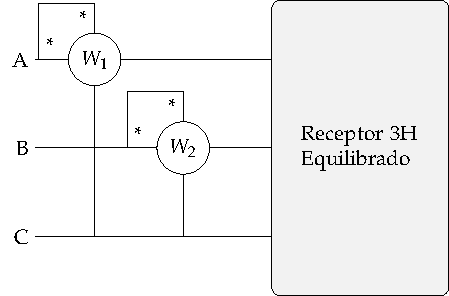
\includegraphics[width=.9\linewidth]{../figs/Potencia3H_Equilibrado_AB.pdf}
\end{center}
\begin{align*}
  W_1&: AC \notin SFD\\
  W_2&: BC \in SFD\\
\end{align*}
\end{column}
\begin{column}{0.33\columnwidth}
\begin{center}
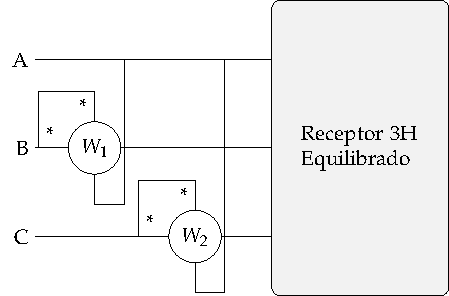
\includegraphics[width=.9\linewidth]{../figs/Potencia3H_Equilibrado_BC.pdf}
\end{center}
\begin{align*}
  W_1&: BA \notin SFD\\
  W_2&: CA \in SFD\\
\end{align*}
\end{column}

\begin{column}{0.33\columnwidth}
\begin{center}
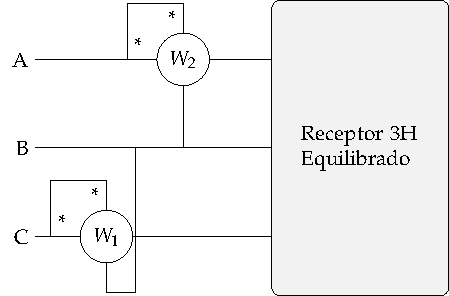
\includegraphics[width=.9\linewidth]{../figs/Potencia3H_Equilibrado_CA.pdf}
\end{center}
\begin{align*}
  W_1&: CB \notin SFD\\
  W_2&: AB \in SFD\\
\end{align*}
\end{column}
\end{columns}
\end{frame}

\begin{frame}[label={sec:org9c374f1},plain]{Otras conexiones: 3H SFI}
\[
  \boxed{(ACB) :: A \triangleright C \triangleright B \Longrightarrow \{AC, CB, BA\}}
\]
\begin{align*}
  W_1 &= UI\cos(\theta - \ang{30}) & P &= W_1 + W_2\\
  W_2 &= UI\cos(\theta + \ang{30}) & Q &= \sqrt{3}(W_1 - W_2)
\end{align*}
\begin{columns}
\begin{column}{0.33\columnwidth}
\begin{center}
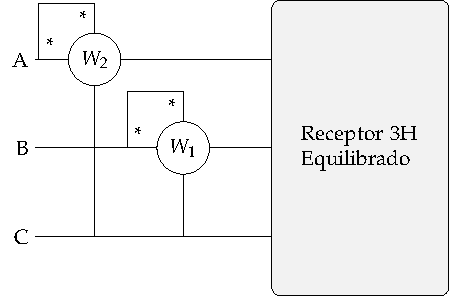
\includegraphics[width=.9\linewidth]{../figs/Potencia3H_Equilibrado_AB_SFI.pdf}
\end{center}
\begin{align*}
  W_1&: BC \notin SFI\\
  W_2&: AC \in SFI\\
\end{align*}
\end{column}
\begin{column}{0.33\columnwidth}
\begin{center}
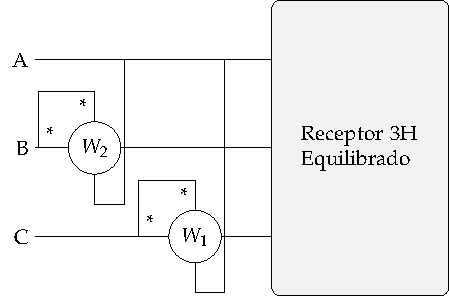
\includegraphics[width=.9\linewidth]{../figs/Potencia3H_Equilibrado_BC_SFI.pdf}
\end{center}
\begin{align*}
  W_1&: CA \notin SFI\\
  W_2&: BA \in SFI\\
\end{align*}
\end{column}

\begin{column}{0.33\columnwidth}
\begin{center}
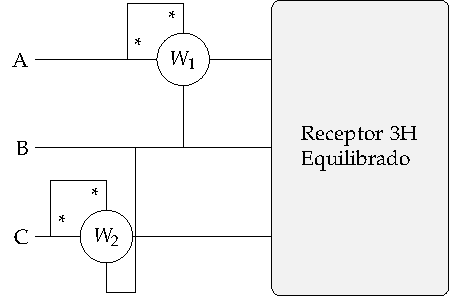
\includegraphics[width=.9\linewidth]{../figs/Potencia3H_Equilibrado_CA_SFI.pdf}
\end{center}
\begin{align*}
  W_1&: AB \notin SFI\\
  W_2&: CB \in SFI\\
\end{align*}
\end{column}
\end{columns}
\end{frame}


\begin{frame}[label={sec:orgccd9a6b}]{Conexiones para medida de reactiva}
\begin{columns}
\begin{column}{0.33\columnwidth}
\begin{center}
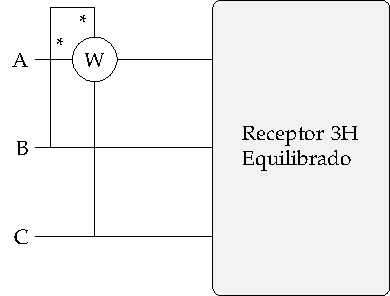
\includegraphics[height=0.25\textheight]{../figs/Reactiva3H_A-BC.pdf}
\end{center}
\[
  W = \Re(\overline{U}_{BC} \cdot \overline{I}_A^*)
\]
\begin{align*}
  BC &\in SFD\\
  BC &\notin SFI
\end{align*}
\end{column}
\begin{column}{0.33\columnwidth}
\begin{center}
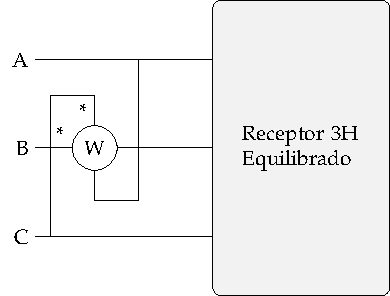
\includegraphics[height=0.25\textheight]{../figs/Reactiva3H_B-CA.pdf}
\end{center}
\[
  W = \Re(\overline{U}_{CA} \cdot \overline{I}_B^*)
\]
\begin{align*}
  CA &\in SFD\\
  CA &\notin SFI
\end{align*}
\end{column}
\begin{column}{0.33\columnwidth}
\begin{center}
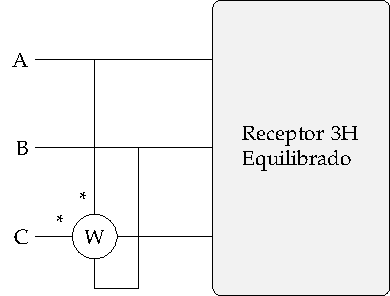
\includegraphics[height=0.25\textheight]{../figs/Reactiva3H_C-AB.pdf}
\end{center}
\[
  W = \Re(\overline{U}_{AB} \cdot \overline{I}_C^*)
\]
\begin{align*}
  AB &\in SFD\\
  AB &\notin SFI
\end{align*}
\end{column}
\end{columns}
\begin{align*}
SFD &\rightarrow \boxed{W = \frac{Q}{\sqrt{3}}}\\
SFI &\rightarrow \boxed{W =  - \frac{Q}{\sqrt{3}}}
\end{align*}
\end{frame}

\begin{frame}[label={sec:orgac54e92}]{Conexiones para medida de reactiva}
\begin{columns}
\begin{column}{0.33\columnwidth}
\begin{center}
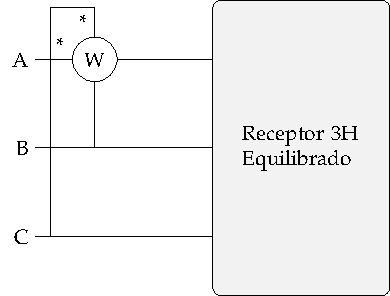
\includegraphics[height=0.25\textheight]{../figs/Reactiva3H_A-CB.pdf}
\end{center}
\[
  W = \Re(\overline{U}_{CB} \cdot \overline{I}_A^*)
\]
\begin{align*}
  CB &\notin SFD\\
  CB &\in SFI
\end{align*}
\end{column}
\begin{column}{0.33\columnwidth}
\begin{center}
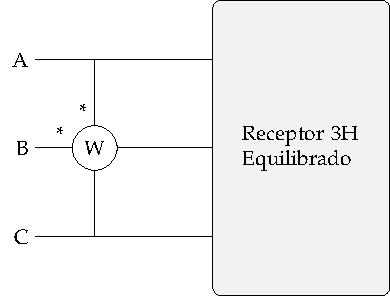
\includegraphics[height=0.25\textheight]{../figs/Reactiva3H_B-AC.pdf}
\end{center}
\[
  W = \Re(\overline{U}_{AC} \cdot \overline{I}_B^*)
\]
\begin{align*}
  AC &\notin SFD\\
  AC &\in SFI
\end{align*}
\end{column}
\begin{column}{0.33\columnwidth}
\begin{center}
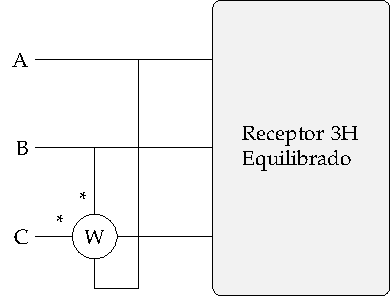
\includegraphics[height=0.25\textheight]{../figs/Reactiva3H_C-BA.pdf}
\end{center}
\[
  W = \Re(\overline{U}_{BA} \cdot \overline{I}_C^*)
\]
\begin{align*}
  BA &\notin SFD\\
  BA &\in SFI
\end{align*}
\end{column}
\end{columns}
\begin{align*}
SFD &\rightarrow \boxed{W = - \frac{Q}{\sqrt{3}}}\\
SFI &\rightarrow \boxed{W = \frac{Q}{\sqrt{3}}}
\end{align*}
\end{frame}

\begin{frame}[label={sec:orgdd74620}]{Medida de la reactiva con receptor desequilibrado}
\begin{center}
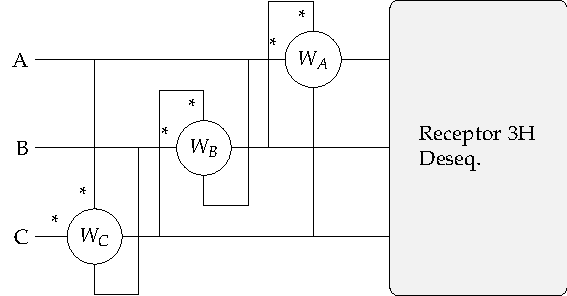
\includegraphics[height=0.5\textheight]{../figs/Reactiva_3H_deseq.pdf}
\end{center}

\begin{columns}
\begin{column}{0.3\columnwidth}
\begin{align*}
  W_A &= \Re(\overline{U}_{BC} \cdot \overline{I}^*_A)\\
  W_B &= \Re(\overline{U}_{CA} \cdot \overline{I}^*_B)\\
  W_C &= \Re(\overline{U}_{AB} \cdot \overline{I}^*_C)        
\end{align*}
\end{column}
\begin{column}{0.3\columnwidth}
\begin{align*}
  \overline{U}_{AB} &= \pm \sqrt{3} \cdot \overline{U}_C \cdot e^{j\pi/2}\\
  \overline{U}_{BC} &= \pm \sqrt{3} \cdot \overline{U}_A \cdot e^{j\pi/2}\\
  \overline{U}_{CA} &= \pm \sqrt{3} \cdot \overline{U}_B \cdot e^{j\pi/2}
\end{align*}
\end{column}
\begin{column}{0.3\columnwidth}
\[
  \boxed{W_A + W_B + W_C = \pm Q/\sqrt{3}}
\]
\end{column}
\end{columns}
\end{frame}
\end{document}